\usetikzlibrary{calc}

\newcommand{\browniank}[6]{% points, delta_t, vol, options, upper, lower
    \pgfmathsetmacro{\picwidth}{#1*#2}
    \begin{scope}
        \draw[#4] (0,0)
            \pgfextra{\pgfmathsetmacro{\cumulativey}{0}}
            \foreach \x in {1,...,#1} {
                let \n1={rand*#3} in 
                \pgfextra{
                    \pgfmathsetmacro{\cumulativey}{\cumulativey + \n1}
                }
                \ifdim \cumulativey pt > #5 pt
                    \breakforeach
                \else
                    \ifdim \cumulativey pt < #6 pt
                        \breakforeach
                    \else
                        -- ++(#2,\n1)
                    \fi
                \fi
            }
        ;
    \end{scope}
}






\begin{center}
    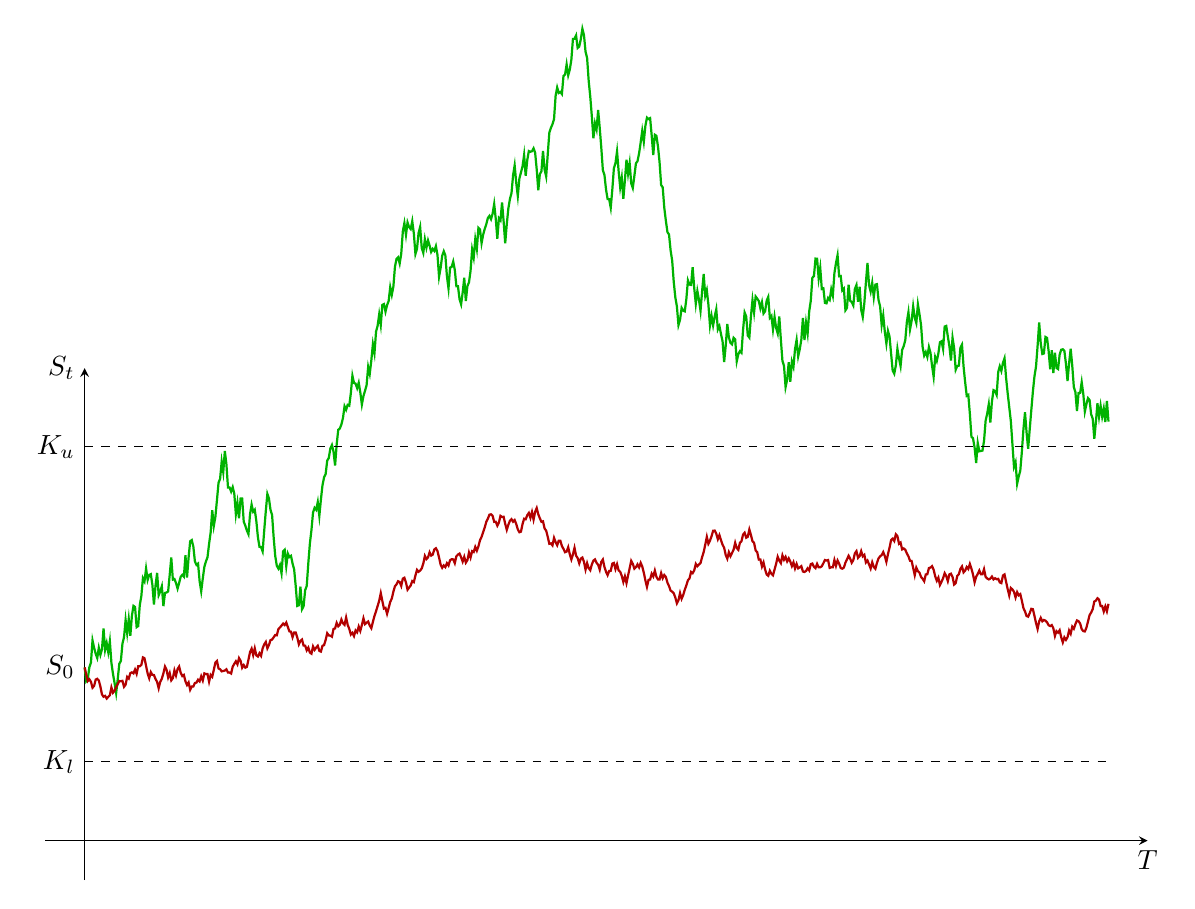
\begin{tikzpicture}[>=stealth]
        % Axes
        \draw[->] (0,-0.5) -- (0,6) node[left] {$S_t$};
        \draw[->] (-0.5,0) -- (13.5,0) node[below] {$T$};

        % Diffusions
        \begin{scope}[shift={(0,2.2)}]
            \browniank{650}{0.02}{0.3}{green!70!black,thick}{2.8}{-1.2}
            \browniank{650}{0.02}{0.1}{red!70!black,thick}{2.8}{-1.2}
        \end{scope}
        
        % Labels
        \node[left] at (0,5) {$K_u$};
        \node[left] at (0,1) {$K_l$};
        \node[left] at (0,2.2) {$S_0$};
        
        % Draw upper barrier
        \draw[dashed] (0,5) -- (13,5);
        % Draw lower barrier
        \draw[dashed] (0,1) -- (13,1);
    \end{tikzpicture}
\end{center}

